\documentclass[12pt]{article}

\usepackage[a4paper, margin=1in]{geometry}
\usepackage{hyperref}
\usepackage{parskip}
\usepackage{graphicx}
\usepackage{float}
\usepackage{fancyhdr}

\hypersetup
{
    colorlinks=true,
    linkcolor=blue,
    urlcolor=blue
}

% Header and footer 
\pagestyle{fancy}
\fancyhf{}
\fancyhead[L]{WhatsWrapped}
\fancyhead[R]{CS-108 Project Report}
\fancyfoot[C]{\thepage}
\renewcommand{\headrulewidth}{0.4pt}
\renewcommand{\footrulewidth}{0.4pt}

\begin{document}

% Title page 

\title{WhatsWrapped,CS108-Project}
\author{Abhinav Verma, Ishan Kumar}
\maketitle
\newpage

% Table of contents
\thispagestyle{empty}
\tableofcontents
\newpage

% Restart page numbering at 1 after TOC so the body starts at page 1
\setcounter{page}{1}

\section{External Libraries}

The project uses a small set of external libraries, kept minimal without using the \texttt{emoji} library so
that the system runs on a clean Python install with almost no setup.

\begin{itemize}
    \item \textbf{numpy} --- used in \texttt{chat.py} for generating probability
    arrays (\texttt{numpy.random.rand}), choosing senders weighted by
    probability (\texttt{numpy.random.choice}), generating message counts
    (\texttt{numpy.random.randint}), and producing the array of dates spanning
    one year (\texttt{numpy.arange} with \texttt{datetime64}).

    \item \textbf{datetime} --- used in both
    \texttt{chat.py} (random time generation, formatting timestamps) and
    \texttt{analyze.py} (parsing timestamps, computing time differences between
    messages, detecting the 12am--4am window for the Night Owl, computing
    response times and the longest silence).

    \item \textbf{json} --- standard library module used in \texttt{analyze.py}
    to write the output \texttt{data.json}, which is the contract between the
    Python parser and the JavaScript front-end.

    \item \textbf{re} --- standard library module used in \texttt{analyze.py}
    to identify emoji code points in \texttt{vocabulary.txt} via a regex over
    the relevant Unicode ranges.

    \item \textbf{sys} --- standard library module used in both Python scripts
    to read command-line arguments (\texttt{sys.argv}).

    \item \textbf{pathlib} --- standard library module used in both
    \texttt{chat.py} and \texttt{analyze.py} to resolve file paths relative
    to the project root, so the scripts work regardless of which directory
    they are invoked from.

    \item \textbf{Chart.js} (\texttt{chart.umd.js}) --- JavaScript charting
    library used in the front-end for the bar charts (Total Messages, Total
    Words, Concise Messenger, Night Owl, Hype Person) and the pie chart
    (group emoji statistics). Loaded as a local script so that no internet
    connection is required at demo time.
\end{itemize}

All other functionality, including the activity heatmap and the slide
navigation, is implemented in plain HTML, CSS and JavaScript.


\section{Design and Architecture}

\subsection{Pipeline}

The Web development was done by Abhinav and the Python was written by Ishan independently.
The project follows the linear pipeline mandated by the specification:

\begin{verbatim}
vocabulary.txt -> chat.py -> chat.txt -> analyze.py -> data.json
                                                          |
                                                          v
                                                       app.js
                                                          |
                                                          v
                                                       Browser
\end{verbatim}

Each stage has a single function and communicates with the next stage
only through a file. This isolation made it easy to develop the Python back-end and the
front-end in parallel. We had decided on a JSON format and worked independently on it.

\subsection{Three Components}

\textbf{Chat Generator (\texttt{chat.py}):} Generates a synthetic year of group
chat messages from a user-supplied vocabulary. The members of the group chat are students who took CS-108 this
semester (\textit{Ishan}, \textit{Abhinav}, \textit{Lokesh}, \textit{Mohan},
\textit{Rishanth}, \textit{Bhanu}, \textit{Rutvik}). The generator assigns
distinct personalities probabilistically rather than deterministically, which
keeps the chat realistic --- the Night Owl can still send a morning message,
just much less frequently.

\textbf{Statistics Parser (\texttt{analyze.py}):} Reads \texttt{chat.txt} line
by line, splits on the fixed format \texttt{DD/MM/YY, HH:MM - Name: message},
and computes both group-level and per-person statistics. The parser does not
``know'' which member was assigned which personality during generation; it
finds the personalities from the \texttt{chat.txt} file alone.

\textbf{Front-End (\texttt{index.html}, \texttt{style.css}, \texttt{app.js}):}
A click-to-advance slideshow with one slide per statistic plus a profile slide.
Slides are absolutely positioned and toggled with an \texttt{active} CSS class;
the only data source is \texttt{data.json}, fetched once on page load. In
addition to the click navigation, keyboard arrow keys (Left / Right) also
advance the slides, and a slide counter (e.g.\ ``5 / 15'') is shown on every
slide so the viewer always knows where they are in the deck.

\subsection{JSON Schema}

The JSON schema separates group-level stats from per-person facts:

\begin{verbatim}
{
  "group_stats": {
    "total_messages_in_chat": int,
    "total_words_in_chat":    int,
    "chat_duration_days":     int,
    "night_owl":              "Name",
    "cncse_msgr":             "Name",
    "chatterbox":             "Name",
    "ghost":                  "Name",
    "conversation_starter":   "Name",
    "selective_responder":    "Name",
    "favourite":              "Name",
    "busiest_day":            "DD/MM/YY",
    "longest_silence":        "Stringified timedelta object",
    "hype_person":            "Name"
  },
  "emoji_stats": { "<emoji>": count, ... },
  "per_person": {
    "Name": {
      "total_messages":         int,
      "total_words":            int,
      "avg_response_time_mins": "X.Y",
      "activity_heatmap":       { "00": int, ..., "23": int },
      "top3_emojis":            [ "<e1>", "<e2>", "<e3>" ]
    },
    ...
  }
}
\end{verbatim}


\subsection{Definition Choices}

Several terms in the specification are left undefined. Our
choices, also written as comments in \texttt{analyze.py}, are:

\begin{itemize}
    \item \textbf{Direct reply / Ghost:} We define the Ghost as the member with
    the highest \emph{streak ratio}: the number of times they send a back-to-back
    message (i.e.\ they sent the previous message and no one replied before
    they sent again), divided by their total messages. Using a ratio rather
    than a raw count prevents the Chatterbox from accidentally winning this
    title just because they send more of everything.

    \item \textbf{Long silence (for Conversation Starter):} We define a long
    silence as a gap of at least one hour between two consecutive messages.
    The Conversation Starter is the member who most often sends the next
    message after such a gap. One hour is short enough that breaks during a
    typical day still count as silences, but long enough to ignore the natural
    pauses inside an active conversation.

    \item \textbf{Average response time:} For every message, if its sender is
    different from the previous sender, we record the time difference as that
    sender's response time; the per-person average is the median of those values,as required by the specification 
    The Hype Person is the member whose mean response time is smallest.
\end{itemize}


\section{Features Implemented}

\subsection{Chat Generation Personalities}

\texttt{chat.py} probabilistically implements the following distinct
personalities. Every personality is enforced through probability arrays
(produced by \texttt{prob\_array}) that are boosted for the relevant member
and re-normalised after each boost.

\begin{itemize}
    \item \textbf{Chatterbox:} The member whose base sender probability is
    highest, given a boost in probability so they remain dominant even
    after later normalisations.

    \item \textbf{Concise Messenger (\textit{cncse\_msgr}):} If the chosen
    sender is this member, the message length is drawn uniformly from
    \texttt{[1, 20]} words; everyone else draws from \texttt{[10, 50]}.

    \item \textbf{Night Owl:} A separate probability array
    (\texttt{nightsender}) is used for messages whose timestamp is between
    \texttt{00:00} and \texttt{04:00}. The Night Owl gets a
    boost in this array.

    \item \textbf{Ghost:} If the previous message's sender is the Ghost, the
    next sender is drawn from \texttt{ghostp\_d} (daytime) or \texttt{ghostp\_n}
    (nighttime), both of which heavily favour the Ghost --- producing the
    streak effect that the parser later detects.

    \item \textbf{Selective Responder + Favourite (custom):} Our custom
    personality. We pick two members, \texttt{sel\_res} and \texttt{fav}.
    The Selective Responder's base probability is \emph{divided} so that they
    normally appear less often, but whenever the previous sender is
    \texttt{fav}, the next sender is drawn from a heavily Selective-Responder-
    biased array. The result: \texttt{sel\_res} is mostly quiet, except
    immediately after \texttt{fav} speaks, when they reply almost every time.
\end{itemize}

The chat spans one full year (\texttt{01-01-2025} to \texttt{31-12-2025}) with a uniformly random number of messages
(0 to 100) per day. Timestamps are generated independently and the entire
list is sorted by \texttt{datetime} before sender selection, so the Ghost
streak and the time-based Night Owl rules operate on a properly ordered chat.

\subsection{Statistics Computed}

\texttt{analyze.py} implements all required statistics plus the custom
ones and a few supporting metrics:

\begin{itemize}
    \item \textbf{total\_messages\_in\_chat / total\_words\_in\_chat} ---
    group totals.
    \item \textbf{chat\_duration\_days} --- number of days from first to last
    message inclusive.
    \item \textbf{chatterbox} --- member with the highest message count.
    \item \textbf{cncse\_msgr} --- member with the lowest words-per-message
    ratio.
    \item \textbf{night\_owl} --- most frequent sender between 00:00 and 04:00.
    \item \textbf{ghost} --- member with the highest streak ratio
    (consecutive same-sender messages divided by their total messages).
    \item \textbf{conversation\_starter} --- most frequent first sender after
    a $\geq$1 hour silence.
    \item \textbf{selective\_responder} and \textbf{favourite} (custom) ---
    the member whose previous-sender distribution is most skewed toward a
    single other member, and who that other member is.
    \item \textbf{busiest\_day} --- date with the highest message count.
    \item \textbf{longest\_silence} --- largest gap between consecutive
    messages.
    \item \textbf{hype\_person} --- member with the smallest average response
    time.
    \item \textbf{Per-person} --- total messages, total words, average response
    time in minutes, top three emojis, and a 24-hour activity heatmap.
    \item \textbf{Group emoji statistics} --- a count of how many times each
    emoji from the vocabulary appeared anywhere in the chat.
\end{itemize}


\subsection{Front-End Slideshow}

The \texttt{index.html} file lays out 15 slides in document order. The
\texttt{app.js} module hides all slides except the one whose index matches
\texttt{currentSlide}, and the Next/Back buttons step through them in a
circular fashion (\texttt{(currentSlide + 1) \% slides.length}). The slides
are:

\begin{enumerate}
    \setcounter{enumi}{-1}
    \item Title slide
    \item Total Messages bar chart (Chart.js).
    \item Total Words bar chart (Chart.js).
    \item Chatter Box reveal.
    \item Concise Messenger reveal with an avg-words-per-message bar chart.
    \item Night Owl reveal with a 24-hour group activity bar chart, with
    the 00:00--04:00 bars highlighted in a contrasting colour.
    \item Ghost reveal.
    \item Hype Person reveal with an avg-response-time bar chart, sorted
    fastest-first so the winner is visually obvious.
    \item Conversation Starter reveal.
    \item Selective Responder reveal.
    \item Busiest Day reveal.
    \item Longest Silence reveal.
    \item Group Emoji pie chart (Chart.js).
    \item User Profiles slide --- buttons for each member, click to add a
    profile card (multiple cards can be shown side by side); each card
    contains messages, words, top emojis, average response time, and a
    24-cell activity heatmap rendered with CSS grid and varying alpha.
    Clicking the same button again toggles that profile off.
    \item Closing slide.
\end{enumerate}

The activity heatmap is implemented manually rather than as a Chart.js chart:
each of the 24 hours becomes a small \texttt{div} whose background colour is
\texttt{rgba(204,134,235,$\alpha$)} where $\alpha$ is the hour's message count
divided by the user's busiest hour. Hovering shows a tooltip with the exact
count.

\subsection{Ingenuity}

Beyond the basic requirements, the front-end includes several quality-of-life
touches:

\begin{itemize}
    \item \textbf{Three additional Chart.js graphs} on the Concise Messenger,
    Night Owl and Hype Person slides, so every reveal is paired with a
    visualisation rather than just a name and a tag line.
    \item \textbf{Slide counter} fixed at the top-left (e.g.\ ``5 / 15'')
    that updates on every navigation, so the audience always knows how far
    they are into the wrap.
    \item \textbf{Keyboard navigation:} Left and Right arrow keys advance the
    slideshow in addition to the on-screen buttons.
    \item \textbf{Profile toggle:} the per-member buttons on the User
    Profiles slide work as a toggle --- clicking once adds the profile,
    clicking again removes it, with the active state reflected on the button
    itself, so multiple profiles can be compared side by side.
\end{itemize}


\section{Directory Structure}

\begin{verbatim}
whatsapp-wrapped/
|-- generator/
|   `-- chat.py              # Synthetic chat generator with personalities
|-- parser/
|   `-- analyze.py           # Reads chat.txt, writes data.json
|-- web/
|   |-- index.html           # Slide markup, one <div class="slide"> per slide
|   |-- style.css            # Slide layout, transitions, heatmap grid
|   |-- app.js               # Slide navigation + Chart.js + heatmap rendering
|   |-- chart.umd.js         # Local copy of Chart.js (for it to work offline)
|   |-- arrow-left.svg       # Back-button icon
|   |-- arrow-right.svg      # Next-button icon
|   `-- background.png       # Slide background
|-- report/
|   |-- report.tex           # This document
|   |--FIRST_SLIDE.png       # First slide photo   
|   |--LAST_SLIDE.png        # Last slide photo
|   `-- Makefile             # Builds report.pdf via pdflatex
|-- vocabulary.txt           # Comma-separated words used by chat.py
|-- chat.txt                 # Generated chat (output of chat.py)
|-- data.json                # Computed statistics (output of analyze.py)
`-- README.md                # How to run, JSON schema description
\end{verbatim}


\section{Installation and Setup}

\subsection{Requirements}

\begin{itemize}
    \item Python 3.10 (oldest we checked with) or newer.
    \item \texttt{numpy} (the only non-standard Python dependency). Install
    with:
\begin{verbatim}
pip install numpy
\end{verbatim}
    \item A modern web browser (Chrome, Firefox or Edge).
    \item No internet connection is required at run time --- \texttt{chart.umd.js}
    is bundled locally.
\end{itemize}

\subsection{Steps to Generate chat.txt and data.json}

\begin{enumerate}
    \item Place a \texttt{vocabulary.txt} file in the project root. It must
    contain comma-separated words; emojis may be mixed in directly.
    \item Generate the chat:
\begin{verbatim}
cd generator
python3 chat.py vocabulary.txt
cd ..
\end{verbatim}
    This creates \texttt{chat.txt} in the working directory.
    \item Compute statistics:
\begin{verbatim}
cd parser
python3 analyze.py chat.txt
cd ..
\end{verbatim}
    This creates \texttt{data.json}.
    \item Open the slideshow. Because \texttt{app.js} fetches \texttt{data.json}
    over HTTP, you must serve the \texttt{web/} directory rather than opening
    \texttt{index.html} from disk:
\begin{verbatim}
python3 -m http.server 5500
\end{verbatim}
    Then visit \texttt{http://127.0.0.1:5500/web/index.html} in your browser.
\end{enumerate}

\section{Usage}

Once the local server is running and the page is loaded, the page can be navigated by the two arrow buttons. The Next button advances through the slides, the Back
button returns. The Left and Right arrow keys also navigate the slideshow.

\begin{figure}[H]
\centering
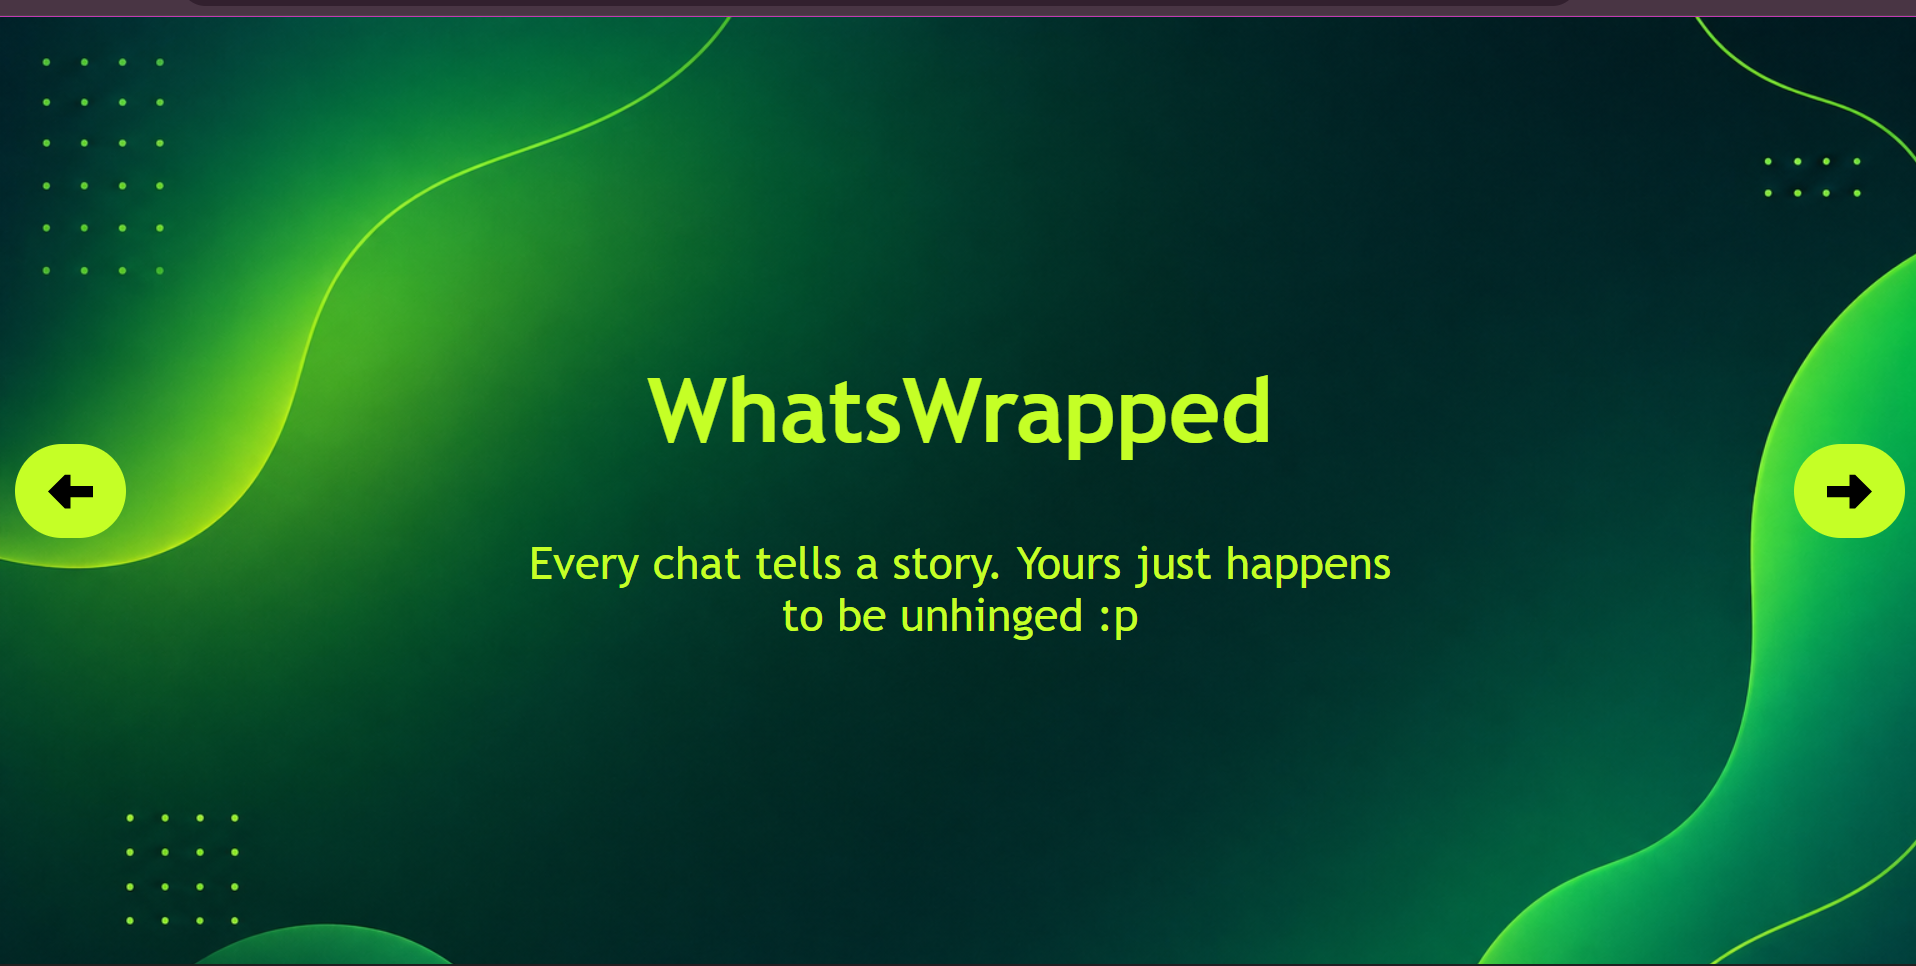
\includegraphics[width=0.85\textwidth]{FIRST_SLIDE.png}
\caption{The opening slide:}
\end{figure}

\begin{figure}[H]
\centering
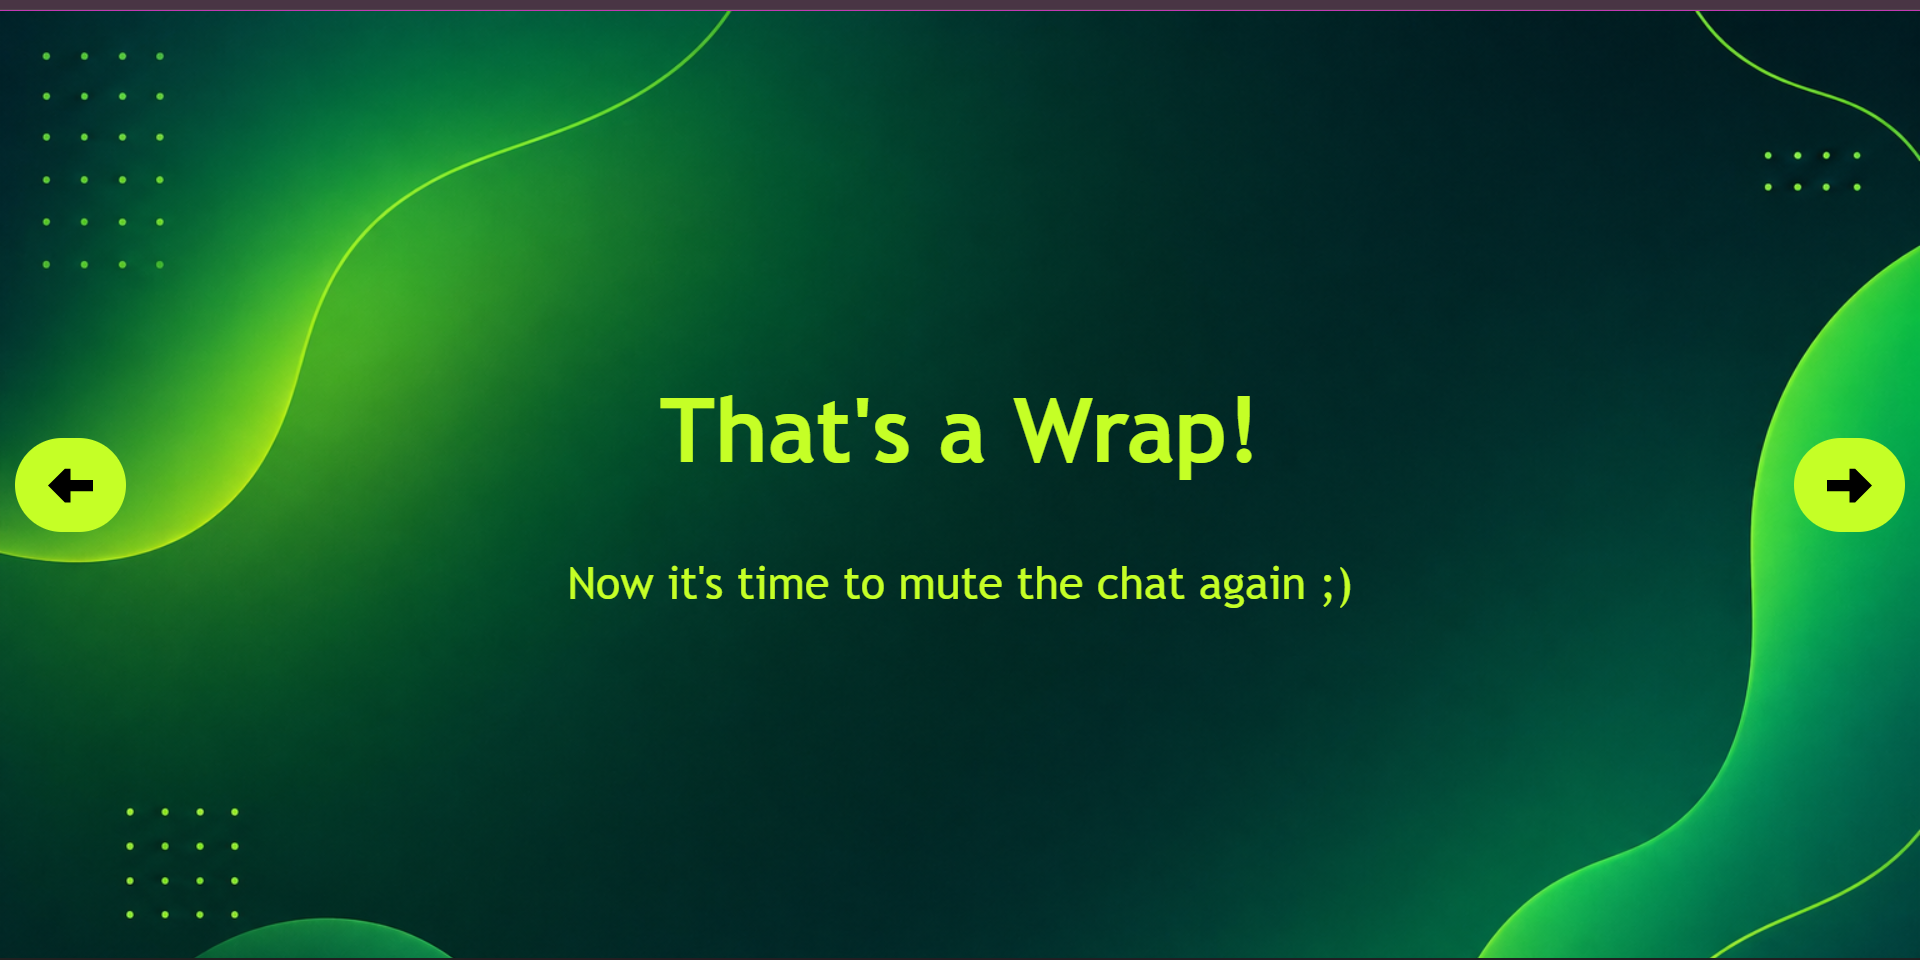
\includegraphics[width=0.85\textwidth]{LAST_SLIDE.png}
\caption{The closing slide:}
\end{figure}

The middle slides reveal each personality (Chatterbox, Concise Messenger,
Night Owl, Ghost, Hype Person, Conversation Starter, Selective Responder)
along with a one-line tag line, and the chart slides show the bar charts and
the emoji pie chart. The User Profiles slide is the only interactive one ---
clicking a member's button adds their profile card to the row, allowing
side-by-side comparisons across multiple members.


\section{Retrospective}

\subsection{Challenges (Python side)}

\textbf{Sorting before sender assignment:} We initially generated each line fully (timestamp + sender + message) before sorting. This broke the Ghost streak, because consecutive lines in time were no longer adjacent in the list. Then, we decided to generate the lines with only timestamp, sort that and only then add sender and message content in it.

\textbf{Tuning probabilities:} The logic that we have used in the chat generator relies on a probability array which keeps changing depending on the time and previous sender. Initially, we had in mind that the same person could have multiple slides (like the nightowl being the ghost and so on). But, this was quite difficult to implement in the sense that the traits randomly chosen by the generator were not matching the traits analysed by the parser (Ex: the generator choosing Abhinav as the nightowl and Ishan as the ghost, but the parser finding that Abhinav is both the ghost and the nightowl). After trying to tune the numbers (probabilities) a lot (to no satisfactory level), \textit{we decided to choose distinct members for each personality.}

\textbf{The Chatterbox overpowering everyone:} The chatterbox, by nature was sending a lot of messages, increasing their chances of sending consecutive messages (making them the ghost), sending messages late at night (making them the nightowl) and making them the selective responder just by the sheer number of messages they sent after a so-called favourite person.
For this, we had to use ratios in the analyser to ensure that the personalities found are in agreement to the ones chose by the generator. This was resolved by making different probability arrays for each case and then reducing the chatterbox's probability by  dividing it, wherever it was required.

\textbf{Path resolution at the last moment:} Our original \texttt{chat.py} and
\texttt{analyze.py} opened files using plain relative paths, which meant they
only worked when invoked from one specific directory. When we tried running
the scripts from the project root the way the spec describes, the files were
not found. We fixed this at the last moment by switching to \texttt{pathlib}:
both scripts now walk up to the project root and locate
\texttt{vocabulary.txt}, \texttt{chat.txt} and \texttt{data.json} via
\texttt{Path.rglob}, so the same command works from any directory.

\subsection{Challenges (Web side)}

\textbf{Learning Chart.js:} Neither of us had used Chart.js before this
project. Working out the configurations (the \texttt{type},
\texttt{data}, \texttt{options} structure),the difference between
\texttt{labels} and \texttt{datasets}, and how the \texttt{responsive} and
\texttt{maintainAspectRatio} options interact with the surrounding container
took a fair amount of trial-and-error reading of the documentation before the
charts looked the way we wanted also the \texttt{plugins} including labels,legend,ticks took some time to understand and find out also maintainaspect ratio did some thing that if we did in css file then it will be doubling the width automatically which took a lot of time to understand.

\textbf{CSS sizing, margins and fonts: } This CSS thing took a lot of time just because designing seems to be the most hard part understanding various transitions various options everything fitted in a container margins paddings also fonts how much font-size should be there so that everything fits understand hovering things i also understood about the .svg files 

\textbf{Heatmap from scratch:} Chart.js does not ship with a heatmap chart
type, so the per-person activity heatmap on the profile cards is made
manually in HTML/JS. From the heatmap in the \texttt{data.json} file, we make a small \texttt{div} for each of
the 24 hours whose background uses
\texttt{rgba(204, 134, 235, $\alpha$)} where $\alpha$ is that hour's count
divided by the busiest-hour count. The 24 boxes are laid out in a 12-column
CSS grid. This took a bit more effort than just calling Chart.js, but the
result looks nice.

\textbf{The data.json path:} While creating the web part, we placed the json file inside the web folder for ease of use. But, we had to change it while running the whole project overall.

\textbf{Emoji rendering:} We had to use the unicode in the javascript becuse we thought it may not run in some systems and didn't want to take a risk.

\subsection{What We Would Do Differently With 10 More Hours}

\begin{itemize}
    \item \textbf{Show the Favourite person of the Selective Responder}: Although generated and parsed, we currently have not implemented a way to see the favourite person of the selective responder. It would be fun to add this like an eater egg.
    
    \item \textbf{Improvise the generation logic:} Even though we tried a lot of ways to generate the chat, the current method can be improved upon. For example, sender probability array could be multiplied by multipliers (which are also arrays) then normalised, before sender assignment rather than using multiple arrays.
    
    \item \textbf{Add mentions:} Right now, the vocabulary doesn't have the names of the members in it. We could implement mentions by slightly changing the sender check condition (by changing the excised string so that it is in the form of - <Sender>: instead of just <Sender>).
    
    \item \textbf{Member portraits on profile cards:} An idea to
include each member's photo on their profile card to make the cards feel more
personal, similar to how Spotify Wrapped uses cover art.

\item \textbf{Richer animations:} The current slide transitions use the
basic fade-and-scale we found in the \href{https://www.w3schools.com/css/css3_animations.asp}{Animation} examples. With more time we
would have explored libraries for better animations --- closer to a real
Spotify Wrapped.

\item \textbf{Slide navigation bar:} Right now the only way to reach a
specific slide is to click Next/Back through everything before it (or do the same. A bottom
navigation bar with one button per slide would let viewers
jump directly to any slide.
\end{itemize}

\nocite{*}
\bibliographystyle{plain}
\bibliography{references}

\end{document}
